\subsection{Army Management}

\subsubsection{Expanding with Leftovers \& Expanding Efficiently}

Take a look at these 2 games at Strat MME featuring Greenland \href{https://www.warzone.com/MultiPlayer?GameID=41158515}{in 2 Turns} and \href{https://www.warzone.com/MultiPlayer?GameID=41406836}{in 3 Turns}, in Figures \ref{green2} and \ref{green3}. It is possible in MME's settings to complete Greenland as your first bonus by the end of T2, only if you spawn at the orange circles (Danmark Havn, Nuuk) and only if you commit 10/10 of your deployments in the first two turns. To generalize, in this template a bonus consisting of 6 territories, can be completed by the end of T2 perfectly optimizing your armies.

\begin{figure}[H]
  \centering
  \begin{minipage}[b]{0.48\linewidth}
    \centering
    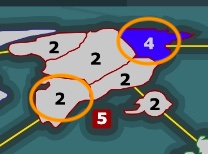
\includegraphics[width=\linewidth, height=7cm]{Images/green2.jpg}
    \caption{Greenland in 2}
    \label{green2}
  \end{minipage}
  \hfill
  \begin{minipage}[b]{0.48\linewidth}
    \centering
    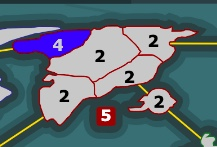
\includegraphics[width=\linewidth, height=7cm]{Images/green3.jpg}
    \caption{Greenland in 3}
    \label{green3}
  \end{minipage}
\end{figure}

To expand on this idea, take a look at this \href{https://www.warzone.com/MultiPlayer?GameID=41533400}{staged game} and Figures \ref{4bon1} and \ref{4bon2}. The two players (call them Black and Ivory from their colours) start building up to a +4 bonus as their first completed bonus. They use a different approach.
\begin{enumerate}
    \item Black splits his deployments on T1, creating a scenario where he will need 2/5 of his deployments on T2 for West Russia. He deploys 3/5 of his deployments on T2 on East USA.
    \item Ivory doesn't stacks in West Africa T1 and needs 3/5 there on T2 to finish the bonus and 2/5 on East China.
\end{enumerate}

The verdict is that in order to complete a +4 bonus as your first bonus in Strat MME, you can go two ways.
\begin{enumerate}
    \item You deploy 7/10 of your income in the first 2 turns to complete it and end up with 2 leftovers in the completed bonus \& 2 elsewhere.
    \item You deploy 8/10 of your income in the first 2 turns to complete it and end up with 3 leftovers in the completed bonus \& 1 elsewhere. 
\end{enumerate}

\begin{figure}[H]
  \centering
  \begin{minipage}[b]{0.48\linewidth}
    \centering
    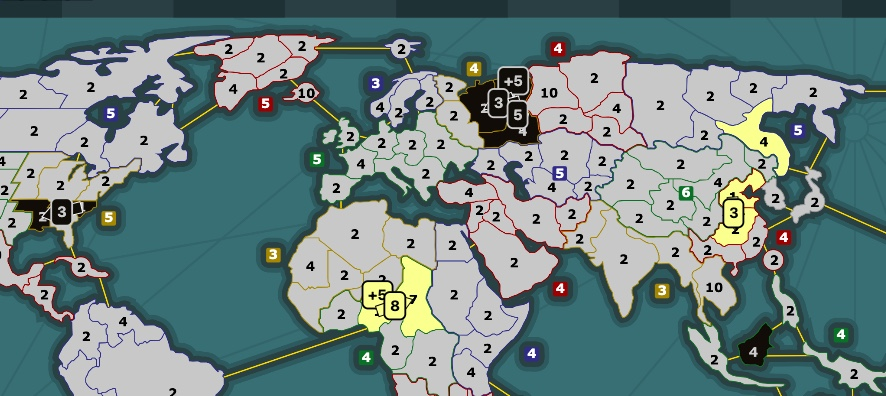
\includegraphics[width=\linewidth, height=4cm]{Images/4bon1.jpg}
    \caption{Turn 1}
    \label{4bon1}
  \end{minipage}
  \hfill
  \begin{minipage}[b]{0.48\linewidth}
    \centering
    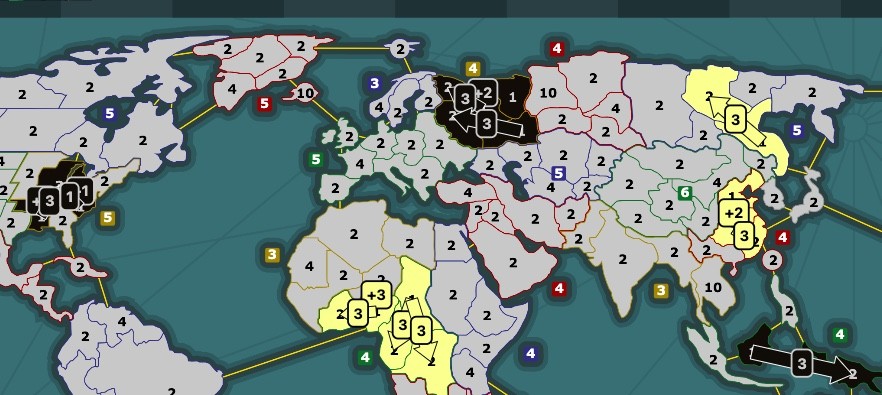
\includegraphics[width=\linewidth, height=4cm]{Images/4bon2.jpg}
    \caption{Turn 2}
    \label{4bon2}
  \end{minipage}
\end{figure}

Whether you go for Ivory's or Black's approach depends on your gameplay and distribution. The Black approach, is more direct, using the least amount of deployments required to finish the project moving into the next one. The Ivory approach can be useful if you suspect things to not work as expect and want a stack just in case. Sometimes you may even want to mix things up in order to leave multiple options open. For example in this \href{https://www.warzone.com/MultiPlayer?GameID=41473232}{Antarctica} game I get 1/2/6, have all the information I can get, but lose the game due to my opponent deploying on T1 in a way that leaves him with multiple options available (ingame chat).
\\
\\
Both Strat MME and Antarctica, the 2 above examples, are vanilla 3x4 templates with 5 income, where expansion isn't so strict - there's a certain level of flexibility in the moves you can play and the order you can capture bonuses. In contrast, in Tarabonia's Choice chaining expansion in a way that allows you to get consecutive bonuses is stricter. For example in this \href{https://www.warzone.com/MultiPlayer?GameID=38142829}{game} Buns goes for 4->4->8->11 and has no room for error. You just cannot afford not splitting and attacking this way, else you'll fall behind in income.
\\
\\
In general, expanding efficiently revolves around a) maximising the usage of your leftover armies and b) not capturing territories you don't need before completing a bonus. However, it's a case-specific idea that changes for template and distribution.

\subsubsection{5vs3 against 3+1vs3}

When looking specifically in trying to capture a 3 army territory, neutral or not, you can quickly see that:
\begin{itemize}
    \item 5vs3 captures and results in 2 leftovers.
    \item A combination of a tap \& a 3vs2 attack captures and results in 1 leftover, as displayed in Figures \ref{5v31} and \ref{5v32}, part of this \href{https://www.warzone.com/MultiPlayer?GameID=40742256}{Guiroma Game}.
\end{itemize}

What's the difference? The idea is using all of your armies in the best way possible. The tap + 3vs2 attack requires 1 less army to setup that you can deploy and have active in another front. While this is especially useful in Guiroma, it can be used against an opponent's stack or to reduce a wasteland. For example:
\begin{itemize}
    \item To kill a 5 army neutral, you can go for 8vs5 or 6vs4 and a tap (7 deployments instead of 8).
    \item To kill a 6 army neutral, you can go for 6vs4 and two taps (8 deployments instead of 10).
    \item To capture a 10-army wasteland, you get in throughout 2 turns by doing 3 taps on T1 and 3 taps + a 6vs4 on T2 (12 deployments instead of 16). And so on.
\end{itemize}

This is analyzed further in the delaying section. 

\begin{figure}[H]
  \centering
  \begin{minipage}[b]{0.48\linewidth}
    \centering
    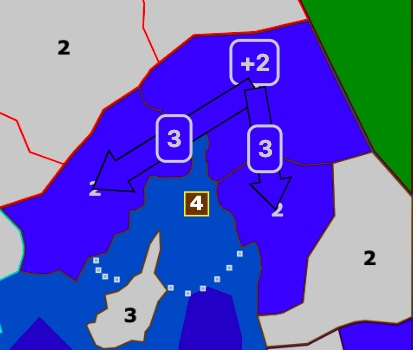
\includegraphics[width=\linewidth, height=6cm]{Images/5v31.jpg}
    \caption{Turn 1}
    \label{5v31}
  \end{minipage}
  \hfill
  \begin{minipage}[b]{0.48\linewidth}
    \centering
    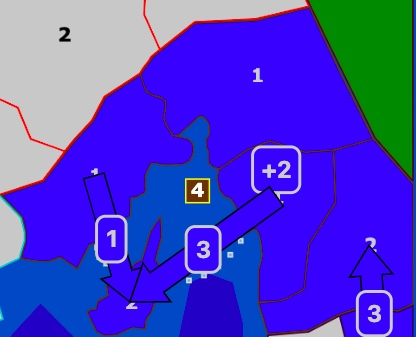
\includegraphics[width=\linewidth, height=6cm]{Images/5v32.jpg}
    \caption{Turn 2}
    \label{5v32}
  \end{minipage}
\end{figure}


\subsubsection{Delaying}

Delaying is something directly correlated with the kill rates of a template. In standard 60:70 kill rates, the defender usually gets a favorable trade. Due to this simple fact, the player attacking usually tries his best to outdelay their opponent, hoping to be the last person on the board to attack. Why? Because attacking after the opponent is better. This can lead to pretty braindead scenario like the one in Figure \ref{delay1}.

\begin{wrapfigure}{r}{0.40\textwidth}
    \centering
    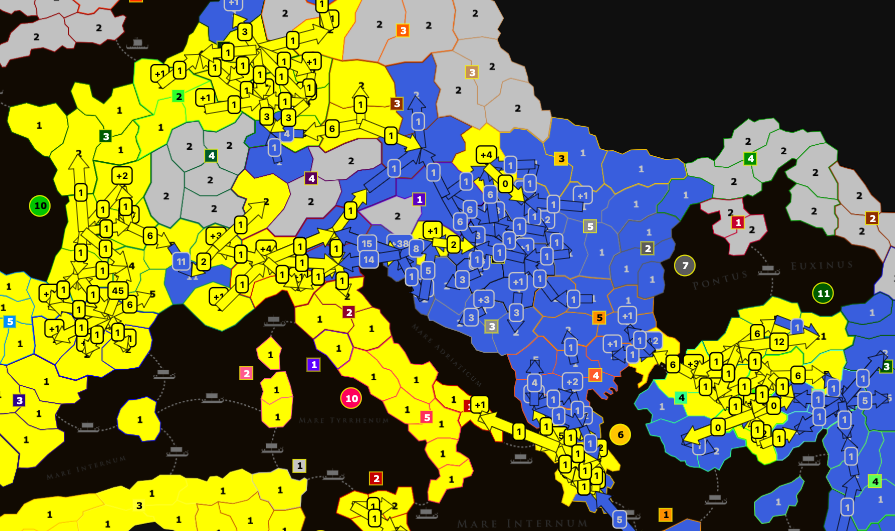
\includegraphics[width=0.40\textwidth]{Images/delaying.png}
    \caption{Embracing your inner delay master}
    \label{delay1}
\end{wrapfigure}

As a concept delaying is particularly weird to understand and comes instinctively. It is very easy to fall into the habit of playing very safe, mass-delaying and attacking on the very last move but that's a) very predictable and b) not the best thing to do more often than not. In fact, if you want to make pretty decent moves drunk at 2am with 1\% battery having forgotten the position, overdelaying and doing a bunch of small attacks is bullet-proof, but lazy and exploitable, while at the end of the day you will never capture back a territory by doing 3-army attacks.
\\
\\

\paragraph{Ability to "Generate" new armies}
%how you can delay +1s and they can attack again
%how you can attack twice with the same armies after getting attacked

In this game there are two very interesting mechanics that you may or may not have noticed yet. Both of them have to do with how armies can sort of multi-attack even when multi-attack is disabled.
\\
\\
The first concept revolves around this sequence:
\begin{enumerate}
    \item I have a front of AvsD armies.
    \item I try transfer $n$ amount of armies to the territory in the front. A -> A+n.
    \item My opponent attacks that territory, from which process I lose some armies.
    \item I out-delay and attack back, using A+n, not just A.
\end{enumerate}

Take for example the following \href{https://www.warzone.com/MultiPlayer?GameID=41232564}{game} and the Figures \ref{f1} to \ref{f5}.

\begin{figure}[H]
  \centering
  % ---------- first image ----------
  \begin{minipage}[b]{0.31\linewidth}
    \centering
    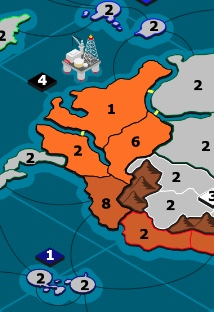
\includegraphics[width=\linewidth,height=5cm]{Images/f1.jpg}
    \caption{Step 1: After deployments}
    \label{f1}
  \end{minipage}
  \hfill
  % ---------- second image ----------
  \begin{minipage}[b]{0.31\linewidth}
    \centering
    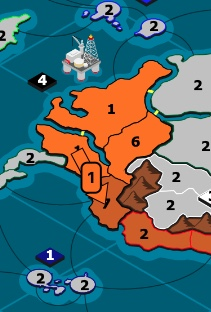
\includegraphics[width=\linewidth,height=5cm]{Images/f2.jpg}
    \caption{Step 2: Opponent Tap}
    \label{f2}
  \end{minipage}
  \hfill
  % ---------- third image ----------
  \begin{minipage}[b]{0.31\linewidth}
    \centering
    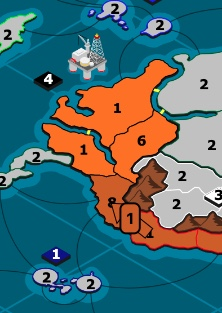
\includegraphics[width=\linewidth,height=5cm]{Images/f3.jpg}
    \caption{Step 3: Transfer 1 army in}
    \label{f3}
  \end{minipage}
\end{figure}

\begin{figure}[H]
  \centering
  % ---------- first image ----------
  \begin{minipage}[b]{0.31\linewidth}
    \centering
    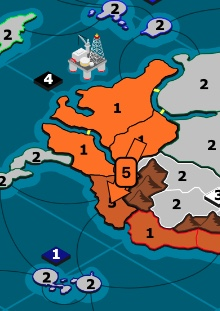
\includegraphics[width=\linewidth,height=5cm]{Images/f4.jpg}
    \caption{Step 4: Opponent attacks }
    \label{f4}
  \end{minipage}
  \hfill
  % ---------- second image ----------
  \begin{minipage}[b]{0.31\linewidth}
    \centering
    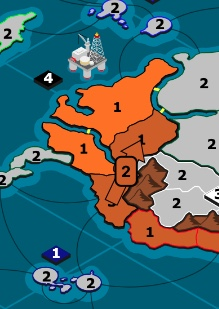
\includegraphics[width=\linewidth,height=5cm]{Images/f6.jpg}
    \caption{Step 5: My first attack}
    \label{f6}
  \end{minipage}
  \hfill
  % ---------- third image ----------
  \begin{minipage}[b]{0.31\linewidth}
    \centering
    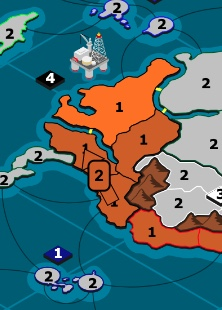
\includegraphics[width=\linewidth,height=5cm]{Images/f5.jpg}
    \caption{Step 6: My second attack}
    \label{f5}
  \end{minipage}
\end{figure}

\begin{itemize}
    \item In the beginning of the turn, I have 7 movable armies in Quito. Figure \ref{f1}
    \item Opponent taps me once, the number of movable armies drops to 6. Figure \ref{f2}.
    \item I transfer one army forward. Intuition says of course armies don't multi attack, that army cannot attack. I am still at 6 movable armies from previous step. Figure \ref{f3}
    \item My opponent attacks with 5, kills 3. My 8 defenders drop to 5. Figure \ref{f4}
    \item I perform two attacks on my last moves, split, 2\&2. Figures \ref{f6} and \ref{f5}.
\end{itemize}

The way I think about this mechanic, is that on step 4, my opponent attacks with 5 and kills 3 of my 8 defenders, including the army I transferred in the same turn. So in reality, my initial 6 movable armies didn't drop down to 3 after the attack, but to 4. The aftermath is that you should be extra careful about how to approach attacking and defending.
\\
\\
The second concept is a continuation of the first one in some way. Above we discussed how when an opponent attacks it acts like killing first the delays you brought in on the same turn before the attack, instead of the initial movable armies. This is about the following sequence, as seen also in Figures \ref{g1} to \ref{g4}.
\begin{enumerate}
    \item I plan 2 split attacks from the same territory to two opponent territories.
    \item I fail to capture an enemy territory, but not all attackers die.
    \item Opponent attacks me on that territory from another territory and kills some armies that survived the first hit.
    \item I attack the second territory with more armies than I should've.
\end{enumerate}

\begin{figure}[H]
  \centering
  \begin{minipage}[b]{0.48\linewidth}
    \centering
    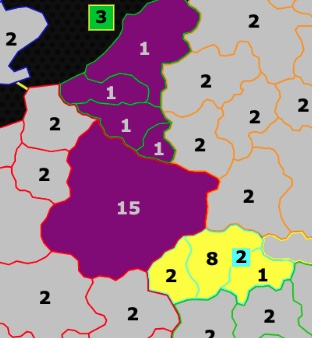
\includegraphics[width=\linewidth, height=6cm]{Images/g1.jpg}
    \caption{Step 1: After deployments}
    \label{g1}
  \end{minipage}
  \hfill
  \begin{minipage}[b]{0.48\linewidth}
    \centering
    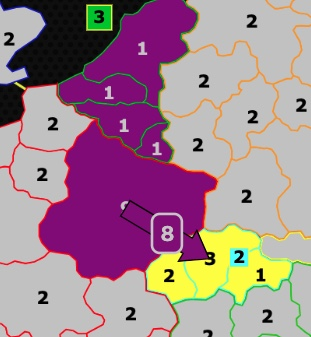
\includegraphics[width=\linewidth, height=6cm]{Images/g2.jpg}
    \caption{Step 2: I queue an attack of 8}
    \label{g2}
  \end{minipage}
\end{figure}

\begin{figure}[H]
  \centering
  \begin{minipage}[b]{0.48\linewidth}
    \centering
    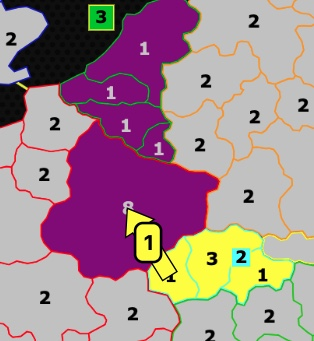
\includegraphics[width=\linewidth, height=6cm]{Images/g3.jpg}
    \caption{Step 3: Tapped from another territory}
    \label{g3}
  \end{minipage}
  \hfill
  \begin{minipage}[b]{0.48\linewidth}
    \centering
    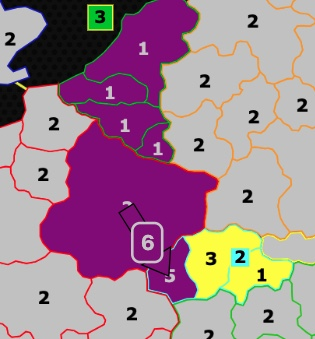
\includegraphics[width=\linewidth, height=6cm]{Images/g4.jpg}
    \caption{Step 4: I queue the second attack of 6}
    \label{g4}
  \end{minipage}
\end{figure}

\begin{itemize}
    \item I deploy up to 15 and plan on doing two attacks of 8 and 6. Figure \ref{g1}.
    \item I queue the first attack of 8, get a 6-, -5 trade. My stack drops from 15 to 9. Figure \ref{g2}.
    \item My opponent taps me from another territory. My stack drops from 9 to 8. Instinctively, this can make you think that the initial attack that I queued with 6 armies, will now be 5 armies, but the tap trades an army from the attackers that survived the first attack. Figure \ref{g3}.
    \item I successfully queue an attack of 6, making it look like I gave birth to an extra army. Figure \ref{g4}.
\end{itemize}

This, as a mechanic, is really hard to take into consideration or utilize in your gameplay. Maybe some times as an attacker you can purposefully have your two attacks in a different cycle in hopes your opponent will attack in between and your armies get some extra value. Or as a defender you have to take into consideration the existence of this mechanic and approach consciously the defense of a double/triple border.

\paragraph{When to delay}
% delay early vs delay late

Generally, if you are a beginner you should delay more, as attacking after your opponent results in a better trade due to the 60/70 kill rate nature. If you've passed the beginner stage, you should start evaluating positions and whether delaying would bring an advantage in the first place.
\\
\\
Furthermore, once you get into the habit of evaluating your position ask yourself am I winning or losing. Delays are a reactionary way of playing the game when defending or when trying to grow an advantage. If you get yourself ahead you should look into converting the position into a win. The very act of converting means finding forcing moves which more often than not don't include extra delays.
\\
\\
To a lot of players I am coming off as a delay-denier so I'm approaching so as to refute them. Delays are further correlated with the idea of having useful armies. Upon evaluating a position it is important to think about the placement of your armies on the board. For example in this \href{https://www.warzone.com/MultiPlayer?GameID=38537237}{game}, by end of Turn 2 the game has the two players on 11vs12 income and 5vs7 useful armies on fronts (with Texx having two extra armies to be brought to the front immediately). By the end of turn 3, the situation is 11vs10 income and 6vs6 useful armies on fronts. The whole circulation of armies you see from turn 4 onwards in the islands +3 bonus is a waste of resources, all starting with wanting to out-delay on turn 3. Always keep in mind 

\paragraph{Army placements and maneuvers}

Generally speaking, you need to have armies that are active. Take a look for example in this \href{https://www.warzone.com/MultiPlayer?GameID=40619054}{BIV game}. I've done some weird things and find myself by the end of Turn 5 at 13vs17 income and down 8 armies in fronts. Borderline a forced loss. However, an army advantage means nothing if your armies are placed in Narnia, which in case was the SW light blue +4 bonus I blockaded and the Green +4 bonus I choose to drop. By the end of Turn 7, I still have an income disadvantage 15vs17, and a glorious army disadvantage of 12vs30 or so, but my opponent threatens nothing and I threaten everything, while his armies won't be useful any time soon. For a similar example, in this \href{https://www.warzone.com/MultiPlayer?GameID=40562183}{Malvia game} by the end of Turn 5 Master USA has an army advantage, yes, but its in the middle of nowhere up north.
\\
\\
Ultimately, this whole section on army management, delays and placements, can be summed up to play for kill-rates, not to outdelay or predict your opponent.

\subsubsection{Conserving armies when attacking}
%on losing armies the more territories you attack

You should always be aware of the fact that even the capture of an 1 army opponent territory will lead to you losing 2 armies in the process. One army from the defensive killrate 1:1 and another army that now becomes locked in place, (1 army stand in guard setting). That's why you'll see better players build stacks in complicated positions and not spread more than they can afford. For example in this \href{https://www.warzone.com/MultiPlayer?GameID=41215348}{Malvia game} I do the exact opposite. Let alone the mistake I did on turn 7 of wasting my stack sending it forward to a territory that doesn't matter, on turn 8 I split attack everything. By the end of turn 7 I have a 22vs1 army advantage locally. By the end of turn 9 I have a 16vs8 army advantage locally (of movable armies). By the and of turn 10 I have a 9vs8 army advantage locally. Do not play like me.

\subsection{Ratio and Stalemates}

\subsubsection{1.7 Ratio and Kill Rates}
When you try to break a territory in 0\% Luck and SR settings, two deterministic tests must both pass, explained in Table \ref{table:break_conditions}.

%---------------- Table A – Conditions to capture & occupy ----------------
\scriptsize
\begin{longtable}{|l|p{8cm}|}
\hline
\rowcolor{Baby_Blue}
Game rule & Deterministic inequality (0 % Luck, SR, 60 %/70 %) \\ \hline\hline
\endfirsthead
\hline
\rowcolor{Baby_Blue}
Game rule & Deterministic inequality \\ \hline\hline
\endhead
\textbf{Kill every defender} & $\mathrm{round}\!\bigl(0.60 \cdot (A-1)\bigr)\;\ge\;D$ \quad\;(\(A-1\) attackers actually move, one stays behind) \\ \hline
\textbf{Keep $\ge 1$ survivor} & $(A-1)\;-\;\mathrm{round}\!\bigl(0.70 \, D\bigr)\;\ge\;1$ \\ \hline
\caption{Two simultaneous conditions that must be met to take a territory}
\label{table:break_conditions}
\end{longtable}
\normalsize

When you solve the first inequality for A you derive approximately. 
$$ A \geq 1.666 \dots D +1 $$

,which is about $1.67 \times D$

The second inequality is milder, producing $A \geq 0.70D + 2$. Once the defenders are above or equal to 4, the 1.67D line is always the higher of the two, so it sets the true break-point. Practically what it means, is that \textbf{if your stack isn't at least 1.7x the defender stack, don't even bother doing detailed math, you cannot break this turn}.

Because both sides are rounded to whole numbers, you often need one or two extra attackers beyond the 1.666 barrier. In practice, the threshold oscillates between 1.67 and 1.83, depending on the remainder classes discussed Tables \ref{table:attackerResidue} and \ref{table:defenderResidue}. So for example in Table \ref{table:rounding_bump} you can see how different defenders require a  higher than 1.67 ratio due to rounding. 

\scriptsize
\begin{longtable}{|c|c|c|c|}
\hline
\rowcolor{Baby_Blue}
Defenders $D$ & Min.\ attackers $A_{\min}$ & Ratio $A_{\min}\! : D$ & Comment \\ \hline\hline
\endfirsthead
\hline
\rowcolor{Baby_Blue}
$D$ & $A_{\min}$ & $A_{\min}\! : D$ & Comment \\ \hline\hline
\endhead
5  & 9  & 1.80 & Rounding forces +2 extra attackers \\ \hline
6  & 11 & 1.83 & Worst-case bump (inefficient 6-stack) \\ \hline
7  & 12 & 1.71 & Drops back toward theoretical $1/0.60 = 1.67$ \\ \hline
8  & 14 & 1.75 & High again (r = 3 class) \\ \hline
9  & 16 & 1.78 & “Hole” at r = 4 \\ \hline
10 & 17 & 1.70 & Almost pure 1.67× bundle \\ \hline
\caption{Minimum attackers required after rounding (0 \% Luck, SR, 60\% / 70\%).  The ratio oscillates around the clean 1/0.60 $\sim$ 1.67 line.}
\label{table:rounding_bump}
\end{longtable}
\normalsize

The 60/70 has been predominantly used for standard settings due to how it creates big enough changes to make this into a more strategic game. 

%-------------- Table C – How kill-rates bend the break-ratio & playstyle --------------
\scriptsize
\begin{longtable}{|c|c|c|c|p{6.5cm}|}
\hline
\rowcolor{Baby_Blue}
Attack rate & Defender rate & “Clean” break-ratio & Practical range & Gameplay Impact \\ \hline\hline
\endfirsthead
\hline
\rowcolor{Baby_Blue}
$p_{\text{atk}}$ & $p_{\text{def}}$ & $1/p_{\text{atk}}$ & Practical ratio & Gameplay Impact \\ \hline\hline
\endhead
0.60 / 0.70 & 0.70 & 1.67 & 1.70 – 1.83 & “Standard.” Fast, tactical; taps \& break-points pay; stalemates rare unless income gap < 2. \\ \hline
0.50 / 0.70 & 0.70 & 2.00 & 2.05 – 2.20 & Slower attack. Many long stalemates; reinforcement cards and +2 income swings decide borders. \\ \hline
0.70 / 0.70 & 0.70 & 1.43 & 1.45 – 1.55 & Buffed offense. Borders melt; initiative beats micro-management; games snowball from offense. \\ \hline
0.40 / 0.50 & 0.50 & 2.50 & 2.55 – 2.70 & Expensive neutral clears; wide maps bog down; No income transition tempo, more about cards and stacks of armies. \\ \hline
\caption{How different kill-rate pairs shift the break-ratio and reshape gameplay on 0 \%-Luck, Straight-Round templates}
\label{table:killrate_variants}
\end{longtable}
\normalsize

At a glance a kill-rate slider looks like a pure numbers tweak, but it actually rewires tempo and pretty much every aspect of strategy one can think of. Think of each template as living on two axes:
\begin{enumerate}
    \item Attacker rate: $p_a$
    \begin{itemize}
        \item Low $p_a$ translates to every battle being a slog, attackers needing huge ratios to move forward. 
        \item High $p_a$ translates to a snow-bally gameplay where the attacker's momentum matters above everything else. The first attack ends the fight.
    \end{itemize}
    \item Defender rate: $p_d$
    \begin{itemize}
        \item Low $p_d$ translates to bonuses that are pretty impossible to defend. Hard to hold gorund, positions crumble.
        \item High $p_d$ translates to a game state where stacks trade away fairly quickly and stalemates form if the players match income.
    \end{itemize}
\end{enumerate}

Mix the two and you get four very broad families.

\begin{enumerate}
    \item Both rates high (e.g. 0.75/0.75 or 1.0/0.9)
    \begin{itemize}
        \item Break ratio at $\approx \frac{1}{p_a} \rightarrow \sim 1.33 \times D$, meaning only 1.33 times the defenders are required to to wipe. 
        \item The end result is borders are fragile, rf cards are likely overkill on top of things, and delaying shouldn't matter. Game becomes about striking fast and often. This translates to wanting to pick small bonuses, rush income, and expect decisive outcomes by as early as Turn 1.
    \end{itemize}
    \item Both rates low (e.g. 0.40/0.50)
    \begin{itemize}
        \item Break ratio rises above $2.5 \times$, even clearing neutrals is now expensive.
        \item This means expansion stalls. It's way slower. Hard draws should appear unless someone secures an income-edge in the long run, while rf cards are important to grow a lead.
        \item Games in theory should last way longer, thus be more positional.
    \end{itemize}
    \item High offense, Low defense (e.g. 0.75/0.50), the Timid Lands case \label{Reverse_Kill_Rates}
    \begin{itemize}
        \item The break ratio is now at $1.33\times D$ which rounds to $\approx 1.35 - 1.45$ with SR bumps.
        \item In reality, the defenders kill 50\% of what they face, so the attacker keeps half their stack to push deeper. The attacker has the advantage. 
        \item Taps don't decide the fight since a simple +1/-1 change rarely affect the fight. 2 attacks become incredibly powerful as 2 attackers kill 2 defenders. 
        \item As a defender sometimes you'd rather out-delay your opponent and attack your own territories for better ratios.
        \item Stalemates don't happen. Wide income-rich maps become viable because you can sprint across empty territories without bogging down. Choke maps lose value, choke-points don't hold. Overall the game becomes more about initiatives, than position and finesse. If you can hit first, do it
    \end{itemize}
    \item Low offense, High defense (e.g. 0.50/0.80)
    \begin{itemize}
        \item Breat ratio explodes past $2.0 \times$ and defenders shred 80\% of what survives. 
        \item Position flips. The game becomes all about choke-points and taps and breakpoints. Pure expansion race stalls, doesn't matter.
        \item Gameplay is highly methodical, puzzle-like. Secure a choke-point, outexpand slowly, or force a break through multi-front pressure or hiding income/armies.
    \end{itemize}
\end{enumerate}

\subsubsection{Stalemates}

If we denote:
\begin{itemize}
    \item A as the attackers before deploys
    \item D as the defenders before deploys
    \item IA, ID the armies each side adds that turn (trasfer ins, income, cards etc)
\end{itemize}

,then after deploys:


\[
\begin{cases}
A' = A + IA - 1 - round(0.70D) \\
D' = D + ID -1 - round(0.60(A+IA-1))
\end{cases}
\]

A hard stalemate occurs when both sides land on a fixed point where 
\[
\begin{cases}
A' = A \\
D' = D
\end{cases}
\]

, which in plain english means, \textbf{The extra armies the attacker brings each turn must be exactly offset by the extra kills the defender scores (and vice versa)}. Take for example this Earthsea \href{https://www.warzone.com/MultiPlayer?GameID=36770903}{game}.
\\
\\
\begin{itemize}
    \item The situation is 5vs1 before deployments
    \item IA = 6, ID = 7
    \item Attacker kills 7, Defender kills 6
    \item Down to 6vs1 again, exactly offsetting the deployments.
\end{itemize}

Another example of it takes place in this \href{https://www.warzone.com/MultiPlayer?GameID=12851727}{Sri Lanka game}, where the position before deployments is 9vs1 at 8vs10 income and the attacker can never break no matter how much they try. due to the 8:10 trade happening every turn.
\\
\\
While these don't happen often, sometimes as the defender this might be your only resort to equalizing the game. Always keep in mind that stalemates will happen when the offset of deployed income is equalized by the offset from the army trade.
\begin{itemize}
    \item 6vs1 armies, 6vs7 income, every trade is 6:7. Attacker deploys one less income every turn, gets +1 defender killed every turn, we go back to the same position at 6vs1.
    \item 1vs9 armies, 10vs8 income, every trade is 8:10
    \item 10vs3 armies, 10vs11 income, attacker sends 19, kills 11. defender kills 10. We end up at 10vs3 again.
    \item 5vs3 armies, 6vs6 income. attacker sends 10, kills 6. defender attacks 6 from his 9, we end up at 5vs3 again. This one though is a soft lock. If the defender taps, he exists the loop and we avoid the stalemate.
\end{itemize}

Lastly, stalemates can occur in INSS templates in situations where both players end up at 0 income unable to move forward, as for example in \href{https://www.warzone.com/MultiPlayer?GameID=33412724}{this} and \href{https://www.warzone.com/MultiPlayer?GameID=17799177}{this}. In general if this ever happens to you in an MTL game, the official guideline is at \href{https://www.warzone.com/Forum/734956-join-multitemplate-ladder-mtl?Offset=44}{this Forum post} where two players vote-to-ended a game. Don't do it, instead find common ground, most likely at remaking the game.
